\section{Results}

In a recent study we have shown that eye movement signals contribute to the perception of body translation, even in the absence of optic flow or a visual fixation point \cite{clemens2015a}. Because eye rotations must be scaled by target depth ($\varphi d = T$) to serve as an adequate translation cue, we tested self-motion perception for near (50 \si{\centi\metre}) and far (200 \si{\centi\metre}) fixations. Participants were presented with two subsequent translation movements \figref{p4:fig1} while they kept fixation on a world- or body-stationary target that was presented either nearby or far away. After the two intervals, they had to judge whether the second translation was longer or shorter than the first.

\begin{figure}
    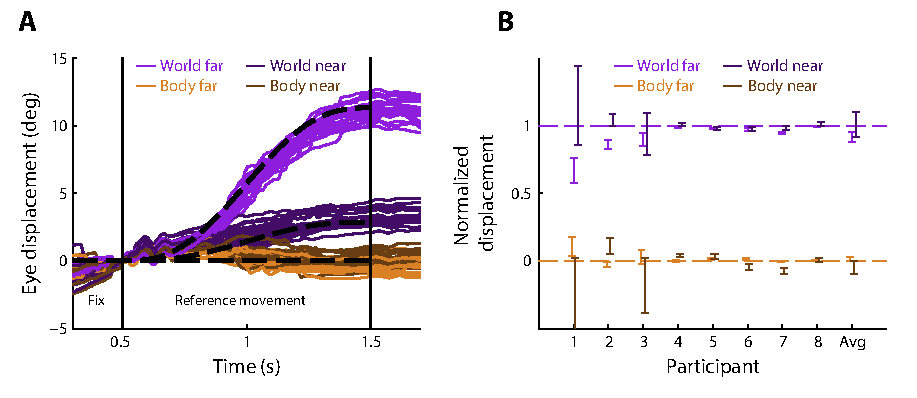
\includegraphics[width=1.0\textwidth]{src/paper4/p4_figure2.pdf}

    \caption{\panelref{A} Actual (solid lines) and ideal (dashed lines) eye movement traces of one participant in the body-fixed (brown and orange) and world-fixed conditions (purple and pink). Gaze was directed at a near (brown and purple) or far (orange and pink) target. All traces shown are for 10m reference movements. \panelref{B} Normalized eye position for each participant (\textpm 95\% confidence interval) at the end of the translation interval for the near and far world fixed targets (purple and pink respectively) as well as the near and far body fixed fixation targets (brown and orange respectively). In addition, the average \textpm SE across all participants is shown. Zero indicates the eyes remained stationary relative to the body, and one indicates the eyes followed the near world fixed target perfectly.}
    \label{p4:fig2}
\end{figure}

We first investigated the ability of participants to fixate body and world stationary targets. \figref{p4:fig2}A depicts exemplar eye traces for the 10cm reference translation with nearby and far fixation points in both the body and world condition. Changes in gaze are largely absent in the body near and body far conditions (brown and orange traces respectively), as required. During the world conditions, the eye movements were large when fixating nearby targets and small when fixating far away ones (purple and pink traces respectively), which reflects the geometrical constraints.

We normalized the eye movement data by taking the average ratio between the measured eye excursion and the geometrically required displacement were the target world stationary. \figref{p4:fig2}B shows that these normalized eye displacements are about zero during body fixed fixations (brown and orange) and close to one in the world fixed fixations (purple and pink data points), for all participants. Our main question is whether these fixation depth dependent differences in eye movements are scaled by fixation depth in order to interpret them as linear self-motion cues.

\begin{figure}
    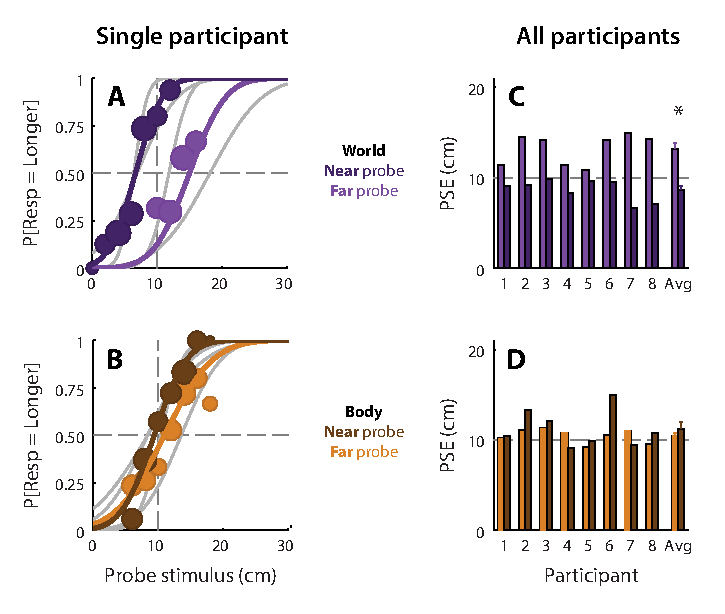
\includegraphics[width=1.0\textwidth]{src/paper4/p4_figure3.pdf}

	\caption{\panelref{A} and \panelref{B} Psychometric curves (colored lines) and associated binned data (circles) for one participant. Circle size represents the amount of trials within the bin. Psychometric curves before collapsing across reference order are shown as gray lines. \panelref{A} Body-fixed condition (brown) while fixation was either near (dark) or far (light). \panelref{B} World-fixed condition (purple) while fixation was either near (dark) or far (light).
	\panelref{C} and \panelref{D} Individual and average points of subjective equality (PSEs). Color scheme matches panels A and B.
	}
	\label{p4:fig3}
\end{figure}

To investigate this question, \figref{p4:fig3} illustrates psychophysical data on self-motion perception of a single participant for the two-fixation depths in both the body (\figref{p4:fig3}A) and world condition (\figref{p4:fig3}B). Lighter and darker colors indicate which fixation depth was the reference translation (see figure legend). The influence of fixation depth is characterized by a shift of the psychometric functions relative to the 10 \si{\centi\metre} reference translation (i.e. the PSE). For example, the rightward shift of the pink curve in \figref{p4:fig3}B, representing the world-condition, means that with a far target a longer translation (\about15 \si{\centi\metre}) was required to be perceived equivalent to a 10 \si{\centi\metre} reference translation with nearby fixation. Likewise, the leftward shift of the purple curve indicates that a shorter translation with near fixation (\about6 \si{\centi\metre}) is required to be perceived the same as the 10 \si{\centi\metre} reference translation with far fixation. Together, these opposite biases suggest that translations are perceived shorter for fixations further away. The brown and orange curves in \figref{p4:fig3}A do not show such shifts, indicating that fixation depth (i.e. near versus far) has no effect in absence of eye movements (i.e. when fixating a body-fixed target during the translation).

Similar results were obtained for all participants, as shown by the individual PSEs (right column of \figref{p4:fig3}). Statistical significance of the effects of fixation depth was evaluated by comparing PSEs for the two fixation depths using a paired t-test. PSEs  differed significantly between the two fixation depths in the world condition, $t(7) = 5.42$, $p < 0.01$ (\figref{p4:fig3}C), but not in the body condition, $t(7) = -1.17$, $p = 0.28$ (\figref{p4:fig3}D), confirming the single subject results (\figref{p4:fig3}A, B). Thus, increasing fixation depth does not influence self-motion perception during body stationary fixations, but causes self-motion to be perceived as shorter during world stationary fixations.

\begin{table}
    \begin{tabular}{l|lll|l}
	Participant & $\alpha_{50}$ & $\alpha_{200}$ & $\frac{d_{200}}{d_{50}}$ & $\alpha$ \\
    \hline
	1 & 0.37 & 0.25 & 1.46 & 0.27 \\
	2 & 0.51 & 0.41 & 1.25 & 0.27 \\
	3 & 0.36 & 0.30 & 1.22 & 0.35 \\
	4 & 0.14 & 0.29 & 0.49 & 0.06 \\
	5 & 0.11 & 0.04 & 2.79 & 0.13 \\
	6 & 0.49 & 0.15 & 3.34 & 0.33\\
	7 & 0.40 & 0.53 & 0.76 & 0.58 \\
	8 & 0.42 & 0.35 & 1.25 & 0.21 \\
    \end{tabular}

    \caption{Best-fit parameter values for 50 and 200 \si{\centi\metre} fixation distances, $\alpha_{50}$ and $\alpha_{200}$ respectively (see \eqnref{p4:eq5}), and their ratio, $\alpha_{200} / \alpha_{50} = d_{200} / d_{50}$, for each participant. Best-fit parameter values, $\alpha$, from our previous paper \protect\cite{clemens2015a} are included for reference.}

    \label{p4:tab2}
\end{table}

\begin{figure}
    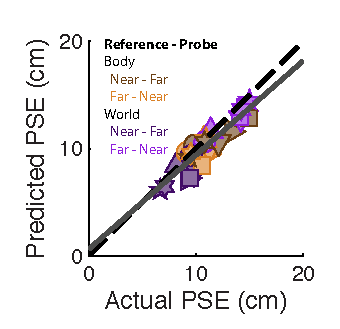
\includegraphics[width=0.5\textwidth]{src/paper4/p4_figure4.pdf}

	\caption{Eye movement based prediction for the PSE plotted against the actual PSE. A data point (symbol) is shown for each participant (symbol shape) and condition (symbol color) pair, following the same color scheme as in \figref{p4:fig3}. The identity line, corresponding to a perfect prediction is shown (solid line) as well as the best fit line (dashed).}
	\label{p4:fig4}
\end{figure}

We used a simple linear model to quantify to what extent eye movements are scaled by fixation depth in order to serve as a linear self-motion cue (see \nameref{p4:sec:methods}). This model describes the perceived translation distance as a weighted average of a vestibular estimate, equal to the actual translation, and an oculomotor-based estimate. The latter estimate depends on the eye excursion which is possibly scaled by fixation depth. We used two weighting parameters, $\alpha_{50}$ and $\alpha_{200}$, one per fixation depth (see \tabref{p4:tab2} for best-fit values). Using these parameters we predicted the PSEs, i.e. $m_p$ in \eqnref{p4:eq5}, and plotted them against the actually observed PSEs in \figref{p4:fig4}. The positive correlation ($\rho = 0.xx$, $p < 0.01$)\footnote{DONT FORGET TO COMPUTE THIS; NEED ACCESS TO MATLAB THOUGH} between observed and predicted PSEs shows that our simple model does reasonably well in predicting perceptual performance.

\begin{figure}
    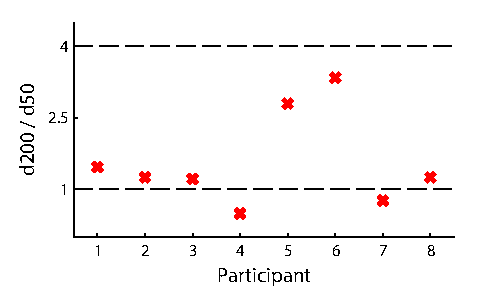
\includegraphics[width=0.5\textwidth]{src/paper4/p4_figure5.pdf}

	\caption{Ratio between near and far parameter values, $\alpha_{200} / \alpha_{50} = d_{200} / d_{50}$ for every participant. Both perfect depth compensation, $\alpha_{200} / \alpha_{50} = 200 / 50 = 4$, as well as the lack thereof, $\alpha_{200} / \alpha{50} = 1$, are represented by a dashed line.}
	\label{p4:fig5}
\end{figure}

By examining the ratio of these weighting parameters, we remove any depth-independent contributions. In absence of  depth scaling, i.e. when $d_{50} = d_{200}$, the ratio should be one. For perfect compensation, that is when $d_{50} = 50  \wedge d_{200} = 200$, the ratio should be $4$. The actual ratio between $d_{50}$ and $d_{200}$ is plotted for each participant in \figref{p4:fig5}. While two participants show moderate compensation for depth, the majority of participants show no sign of scaling of eye movements by fixation distance. This is consistent with the observation that translations are perceived shorter with far compared to near fixations in the world condition.
